\FloatBarrier
\subsubsection{Scalar product method}

\begin{figure}[ht]
    \begin{subfigure}{.49\textwidth}
        \centering
        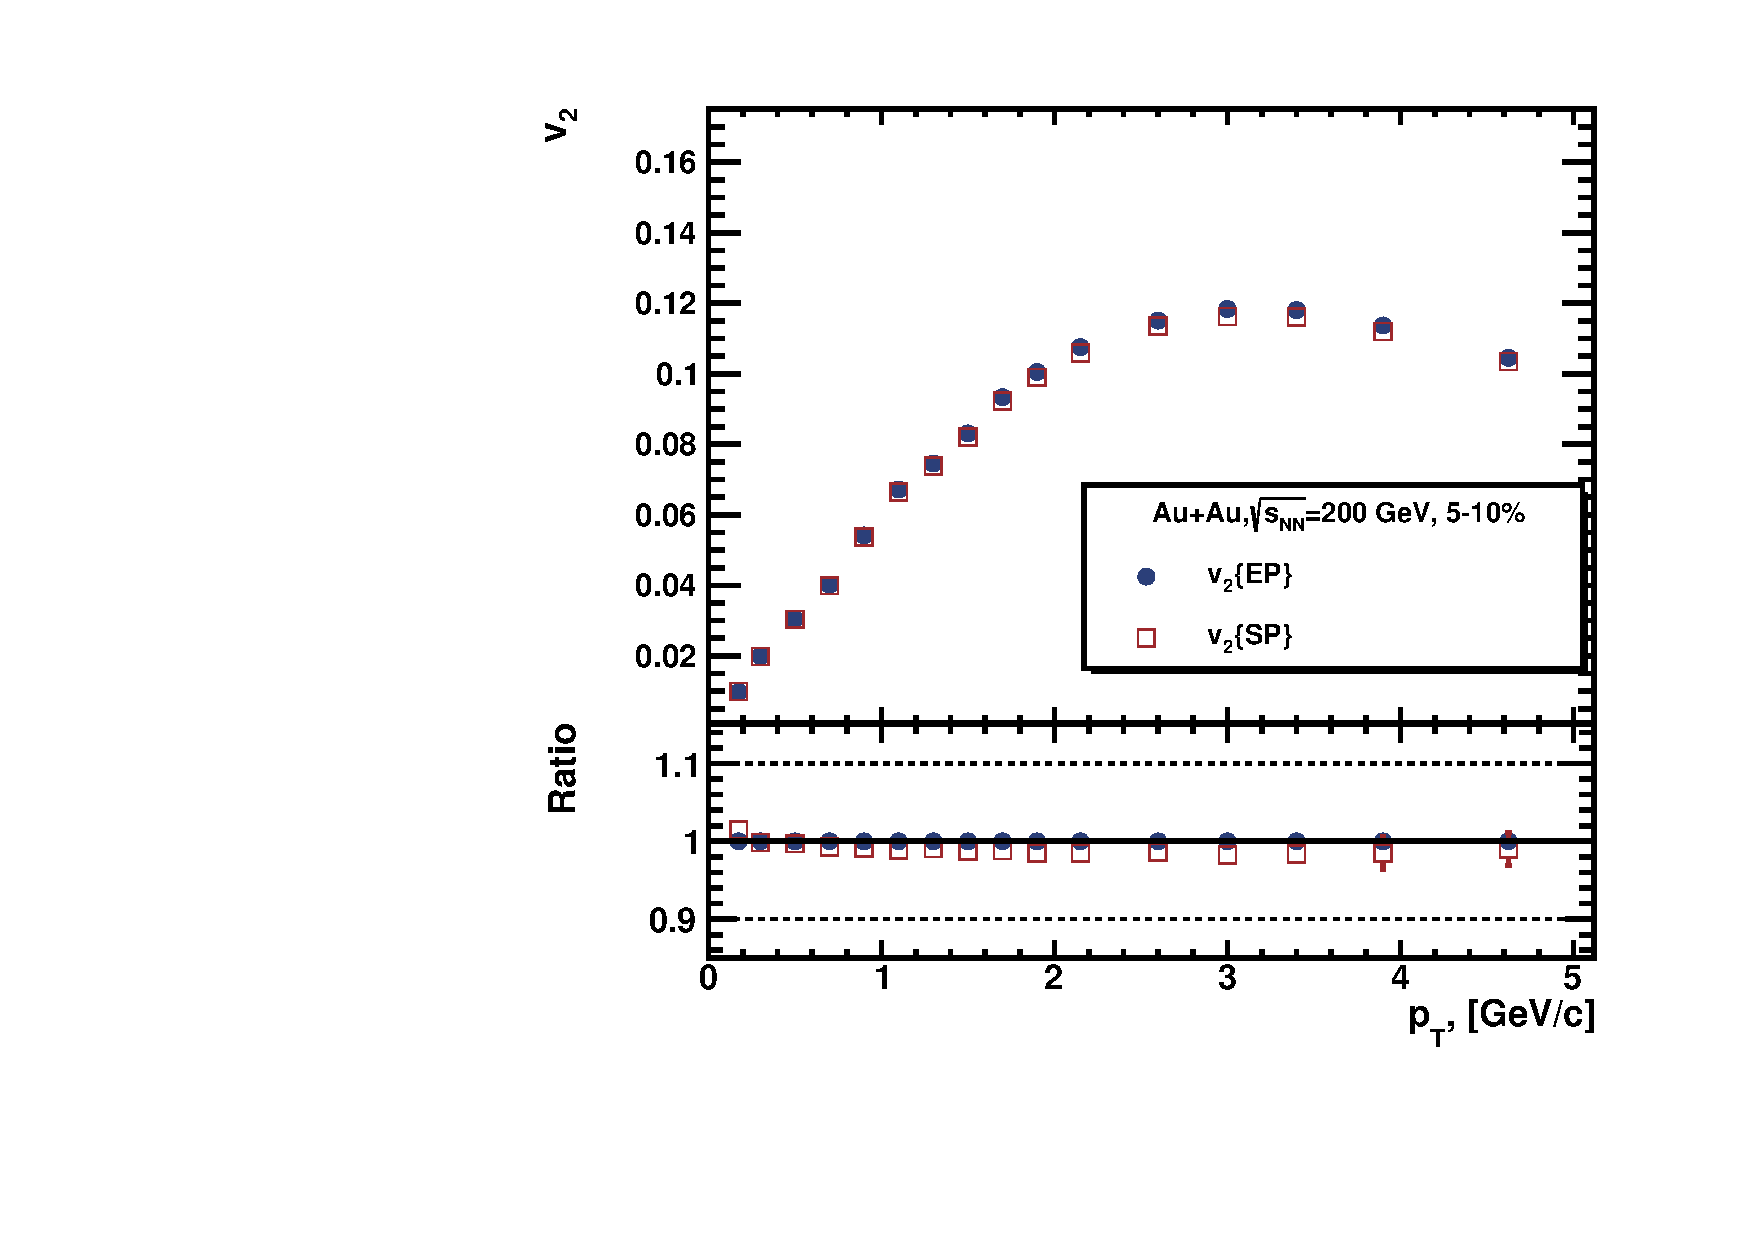
\includegraphics[width=1.\linewidth]{Figures/v2_CH_SP_pt_cent1.pdf}
        %\caption{a}
    \end{subfigure}
    \begin{subfigure}{.49\textwidth}
        \centering
        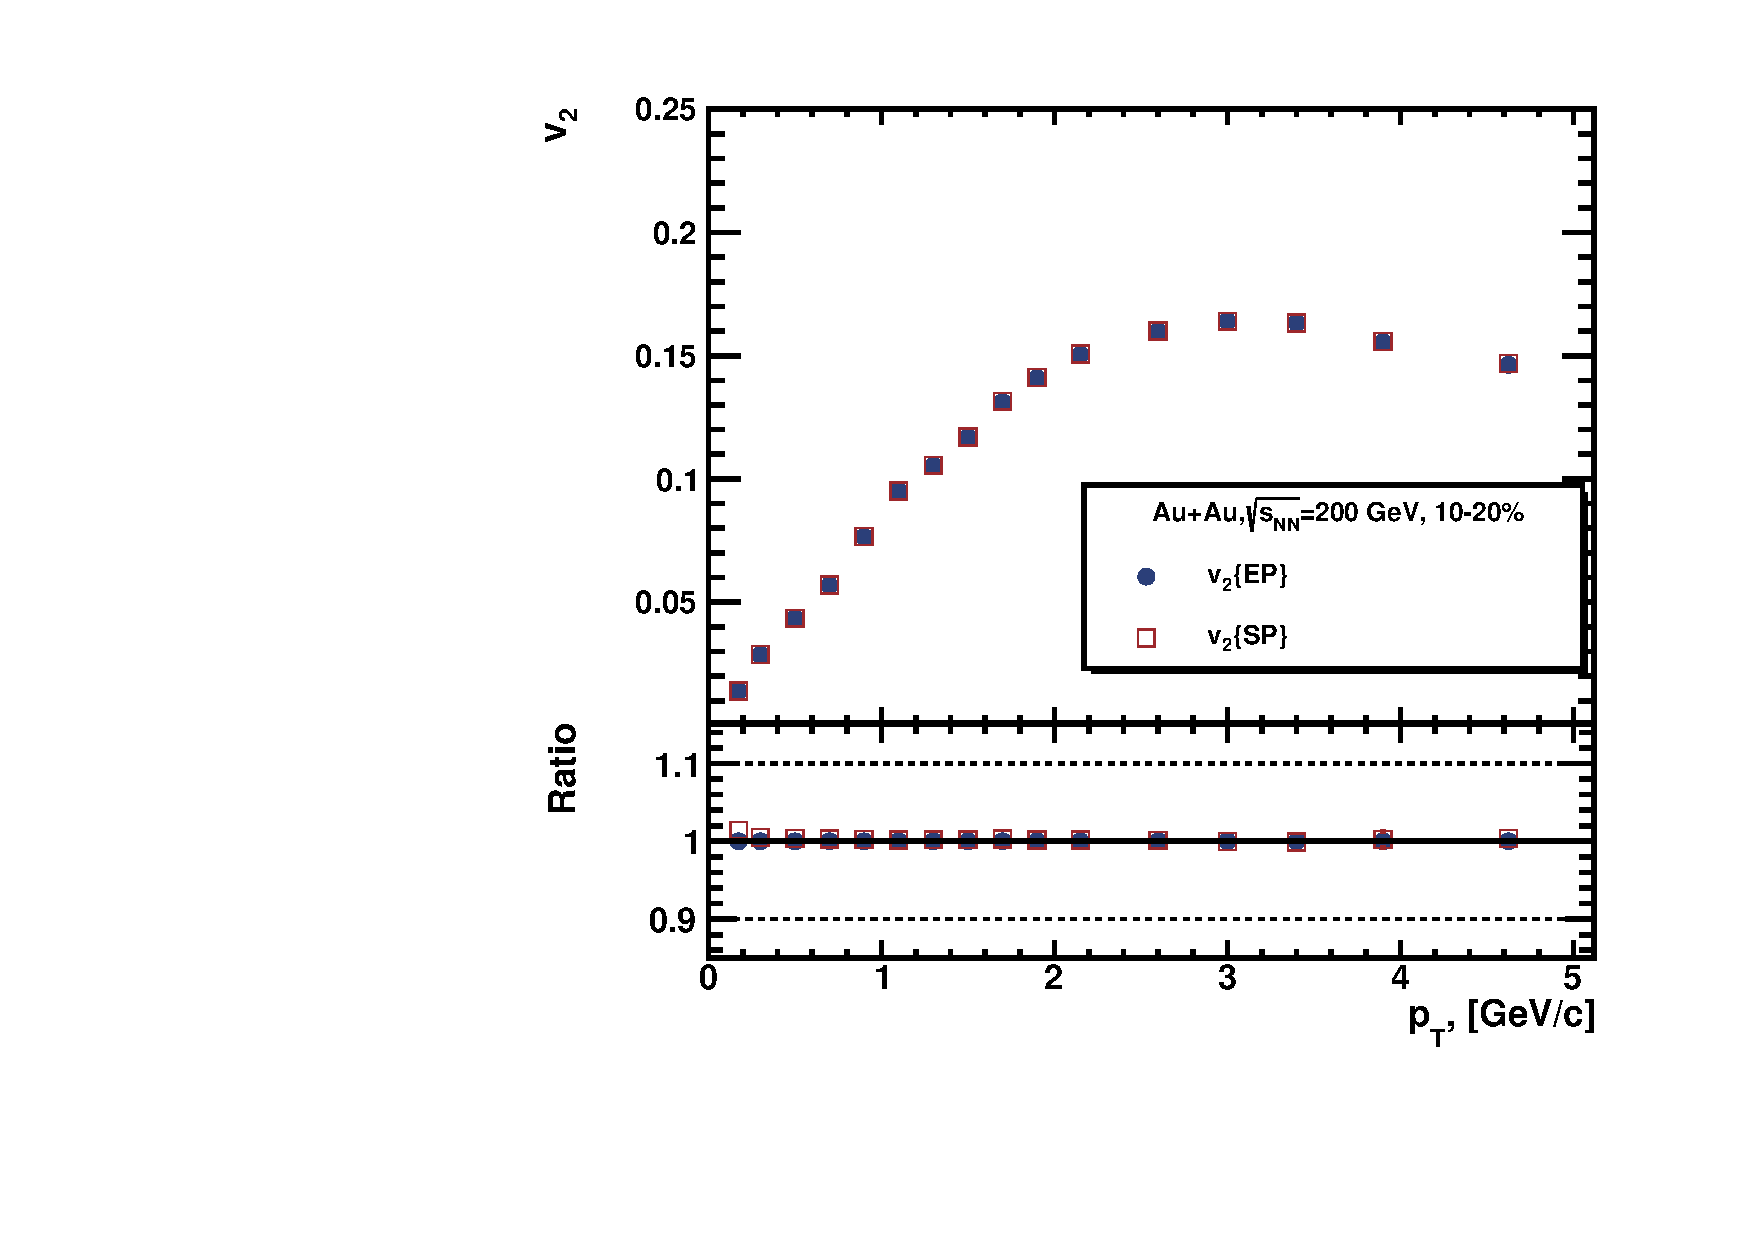
\includegraphics[width=1.\linewidth]{Figures/v2_CH_SP_pt_cent2.pdf}
        %\caption{b}
    \end{subfigure}
    \\
    \begin{subfigure}{.49\textwidth}
        \centering
        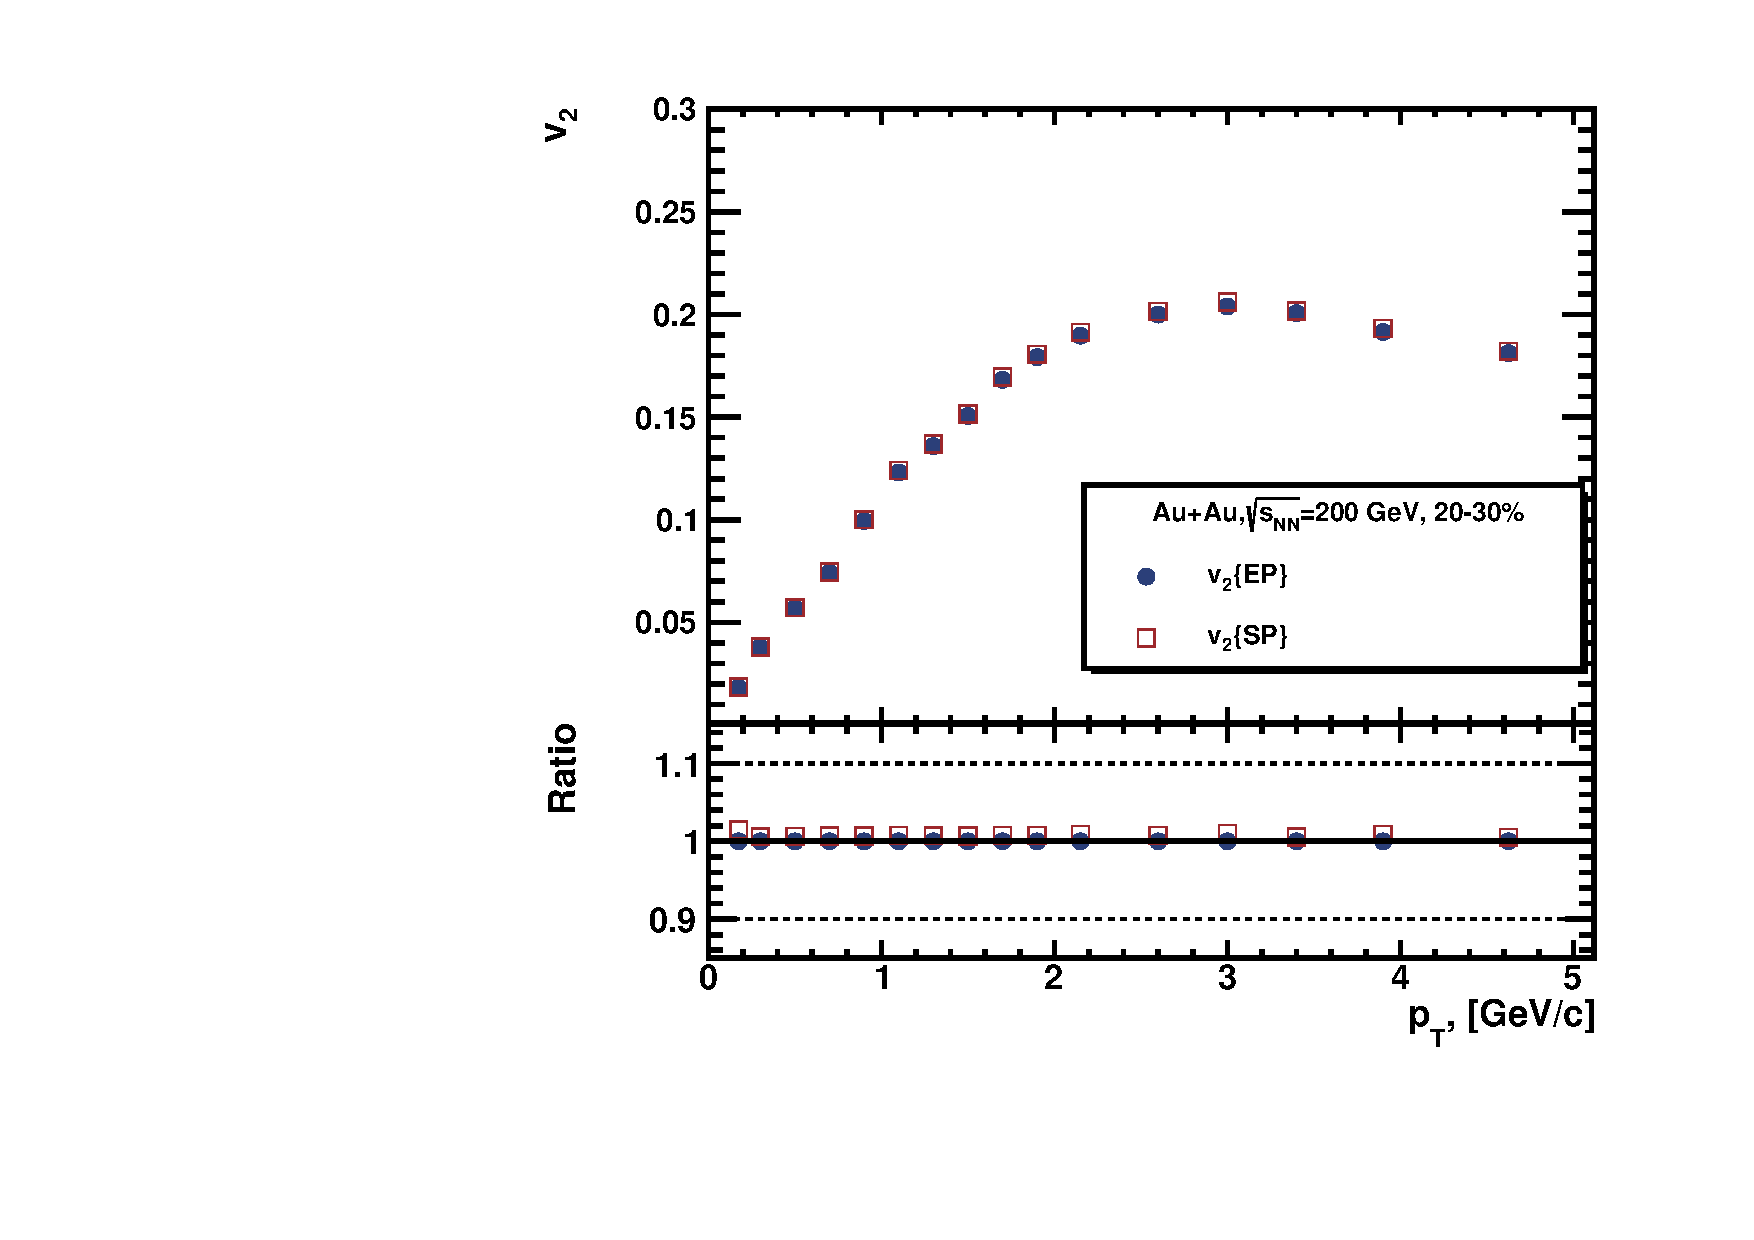
\includegraphics[width=1.\linewidth]{Figures/v2_CH_SP_pt_cent3.pdf}
        %\caption{a}
    \end{subfigure}
    \begin{subfigure}{.49\textwidth}
        \centering
        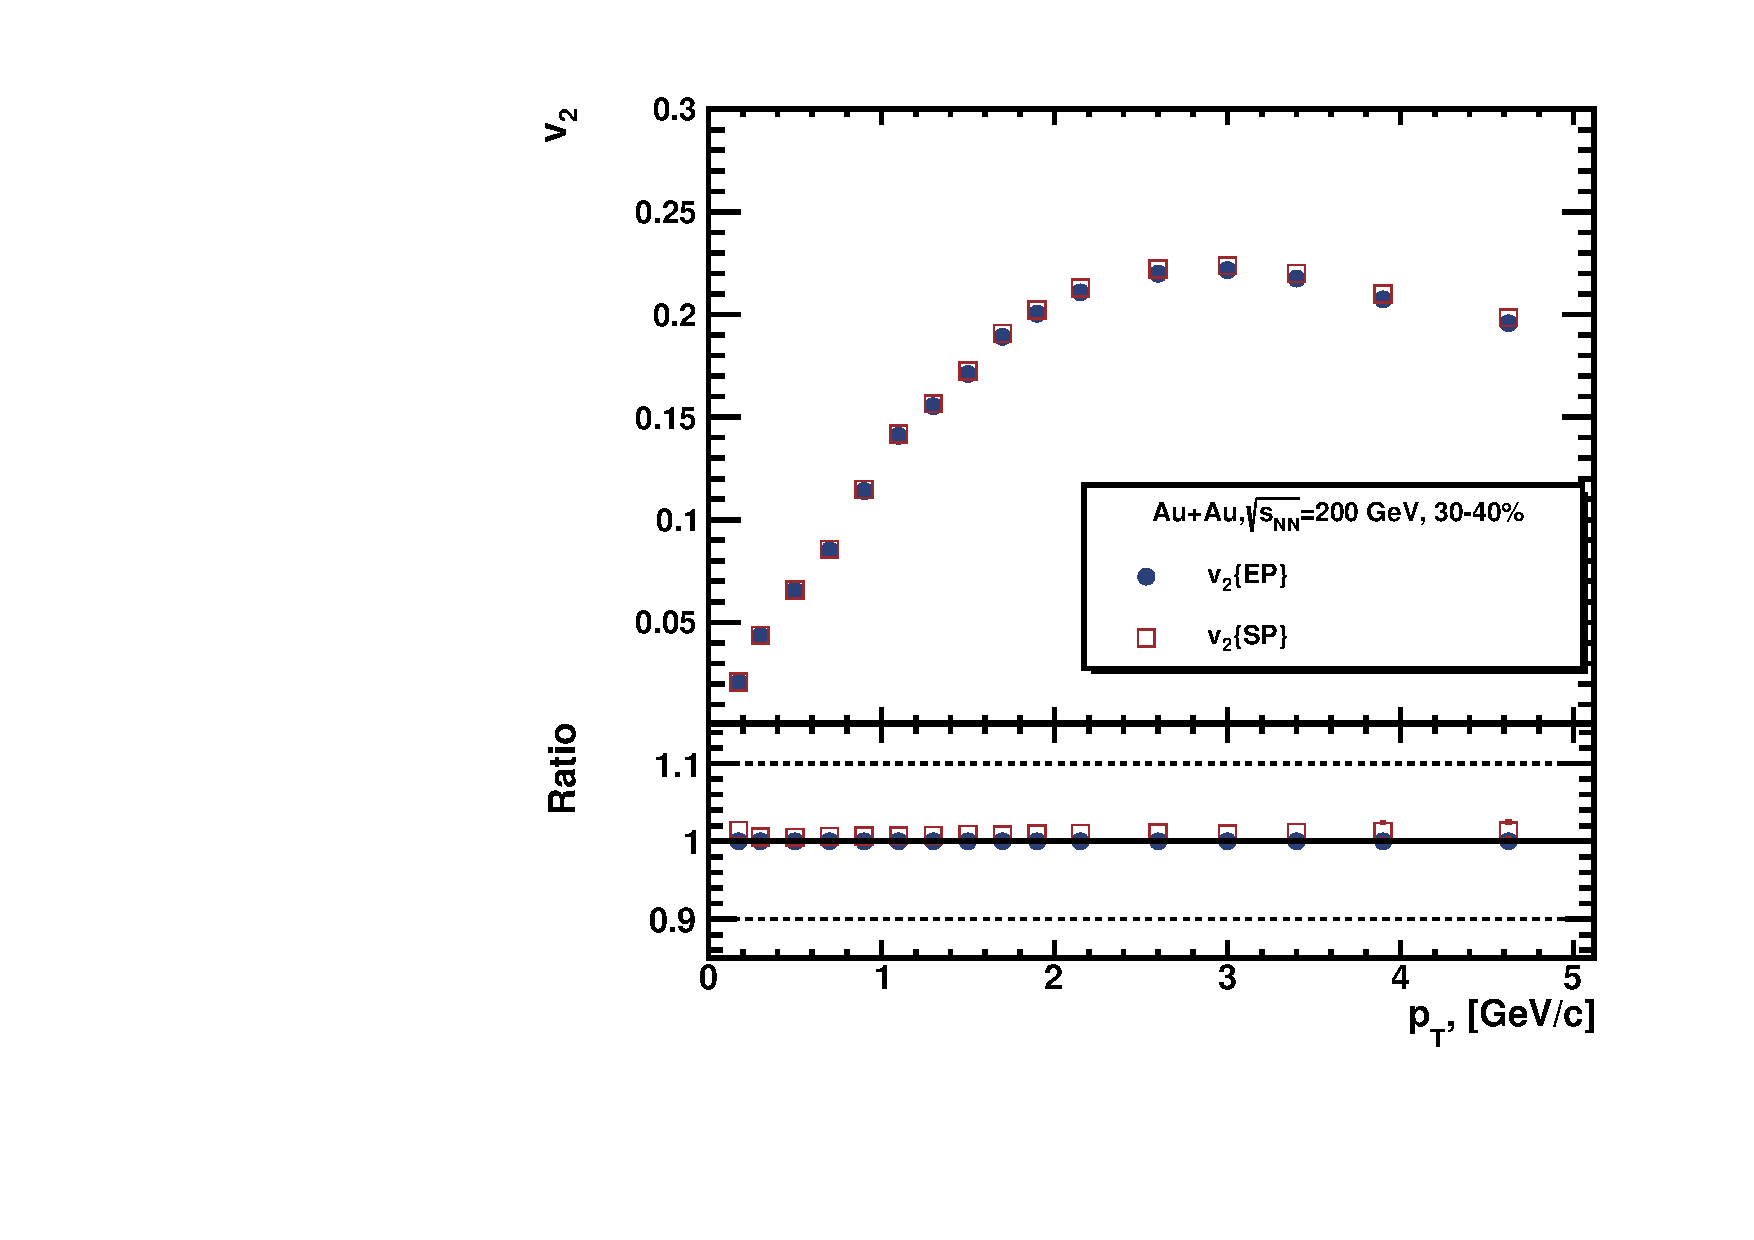
\includegraphics[width=1.\linewidth]{Figures/v2_CH_SP_pt_cent4.pdf}
        %\caption{b}
    \end{subfigure}
    \label{fig:v2_SP_CH}
    \caption{Charged hadron $v_2(p_T)$ for 5-10\% (upper left), 10-20\% (upper right), 20-30\% (bottom left) and 30-40 \% (bottom right) centrality classes in \AuAu\ collisions at \sNN\ = 200 GeV. Results gained with scalar product method were compared with the event-plane ones.}
\end{figure}

\FloatBarrier
\subsubsection{\BBC\ event-plane}

\begin{figure}[ht]
    \begin{subfigure}{.49\textwidth}
        \centering
        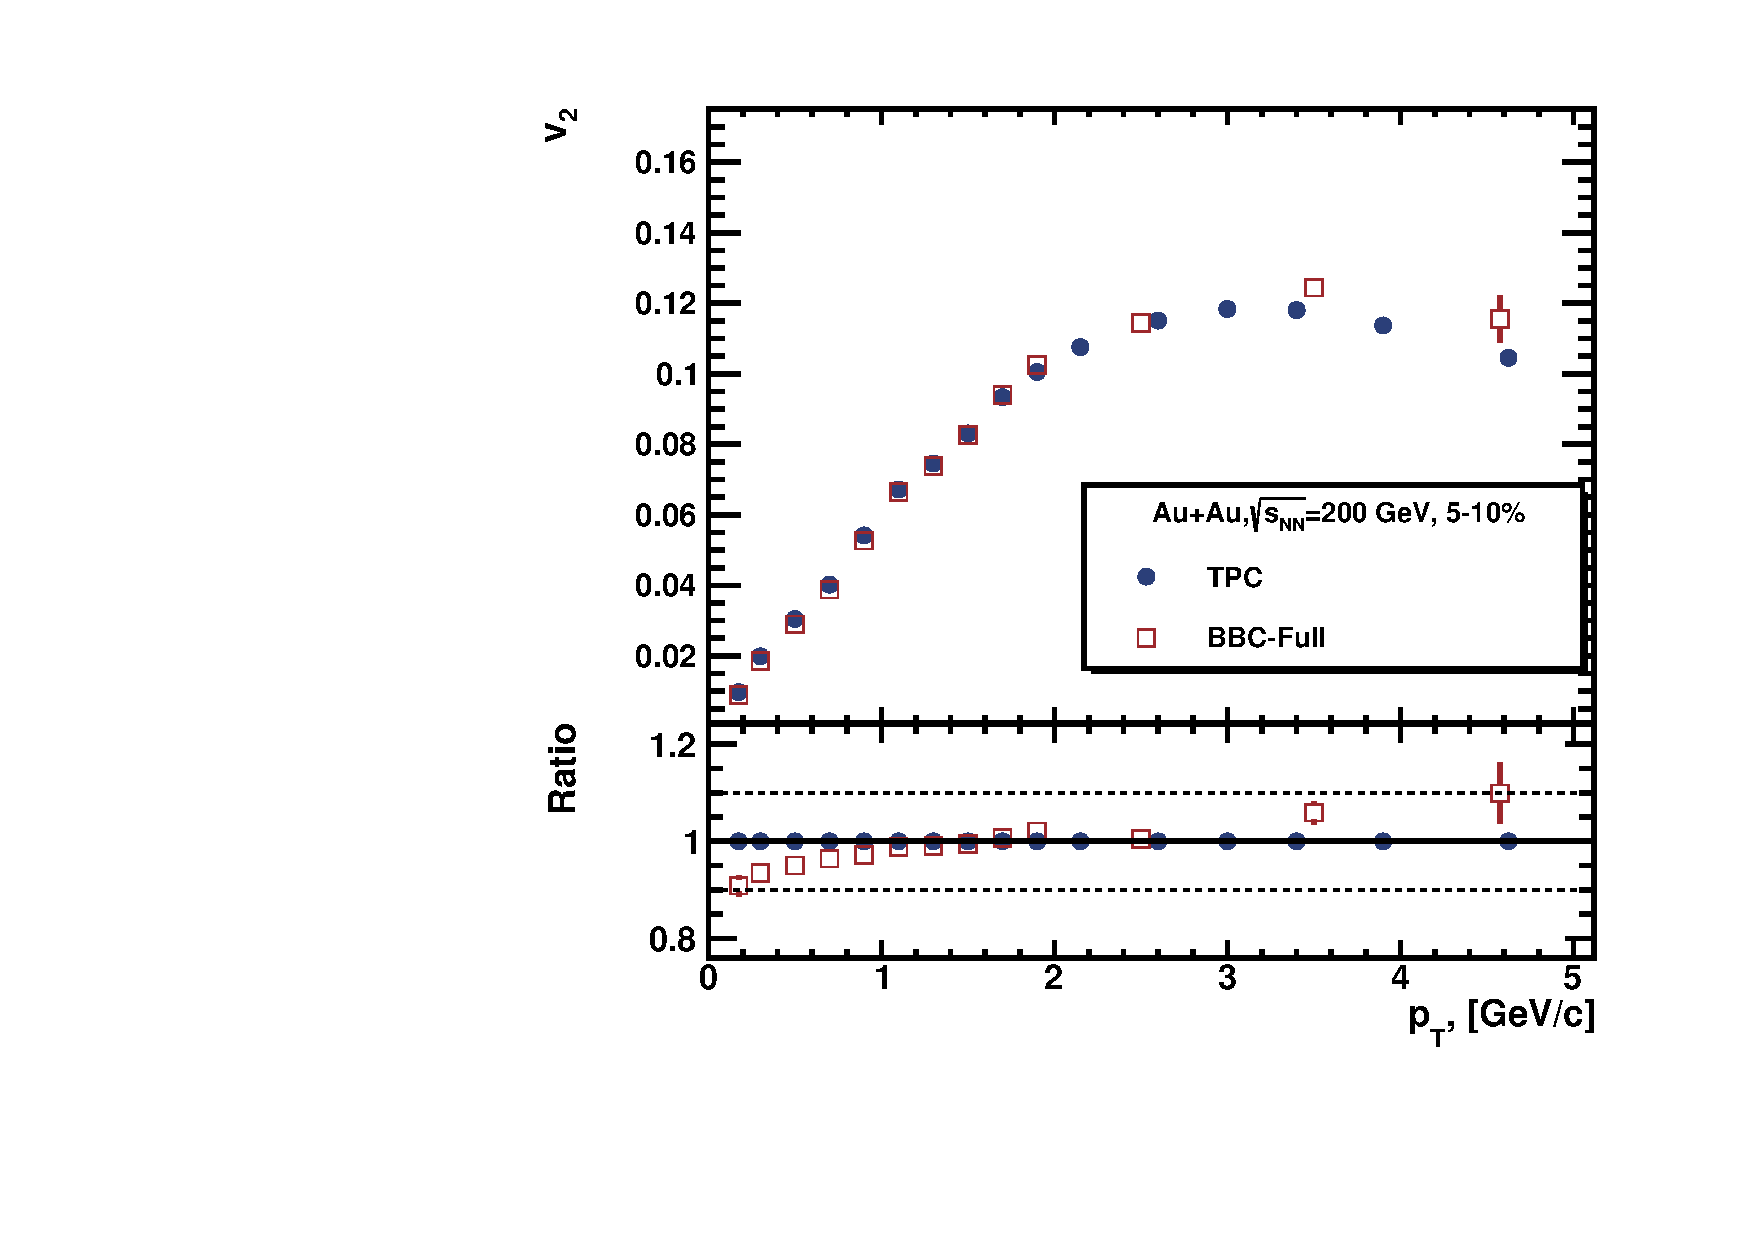
\includegraphics[width=1.\linewidth]{Figures/v2_CH_BBC_pt_cent1.pdf}
        %\caption{a}
    \end{subfigure}
    \begin{subfigure}{.49\textwidth}
        \centering
        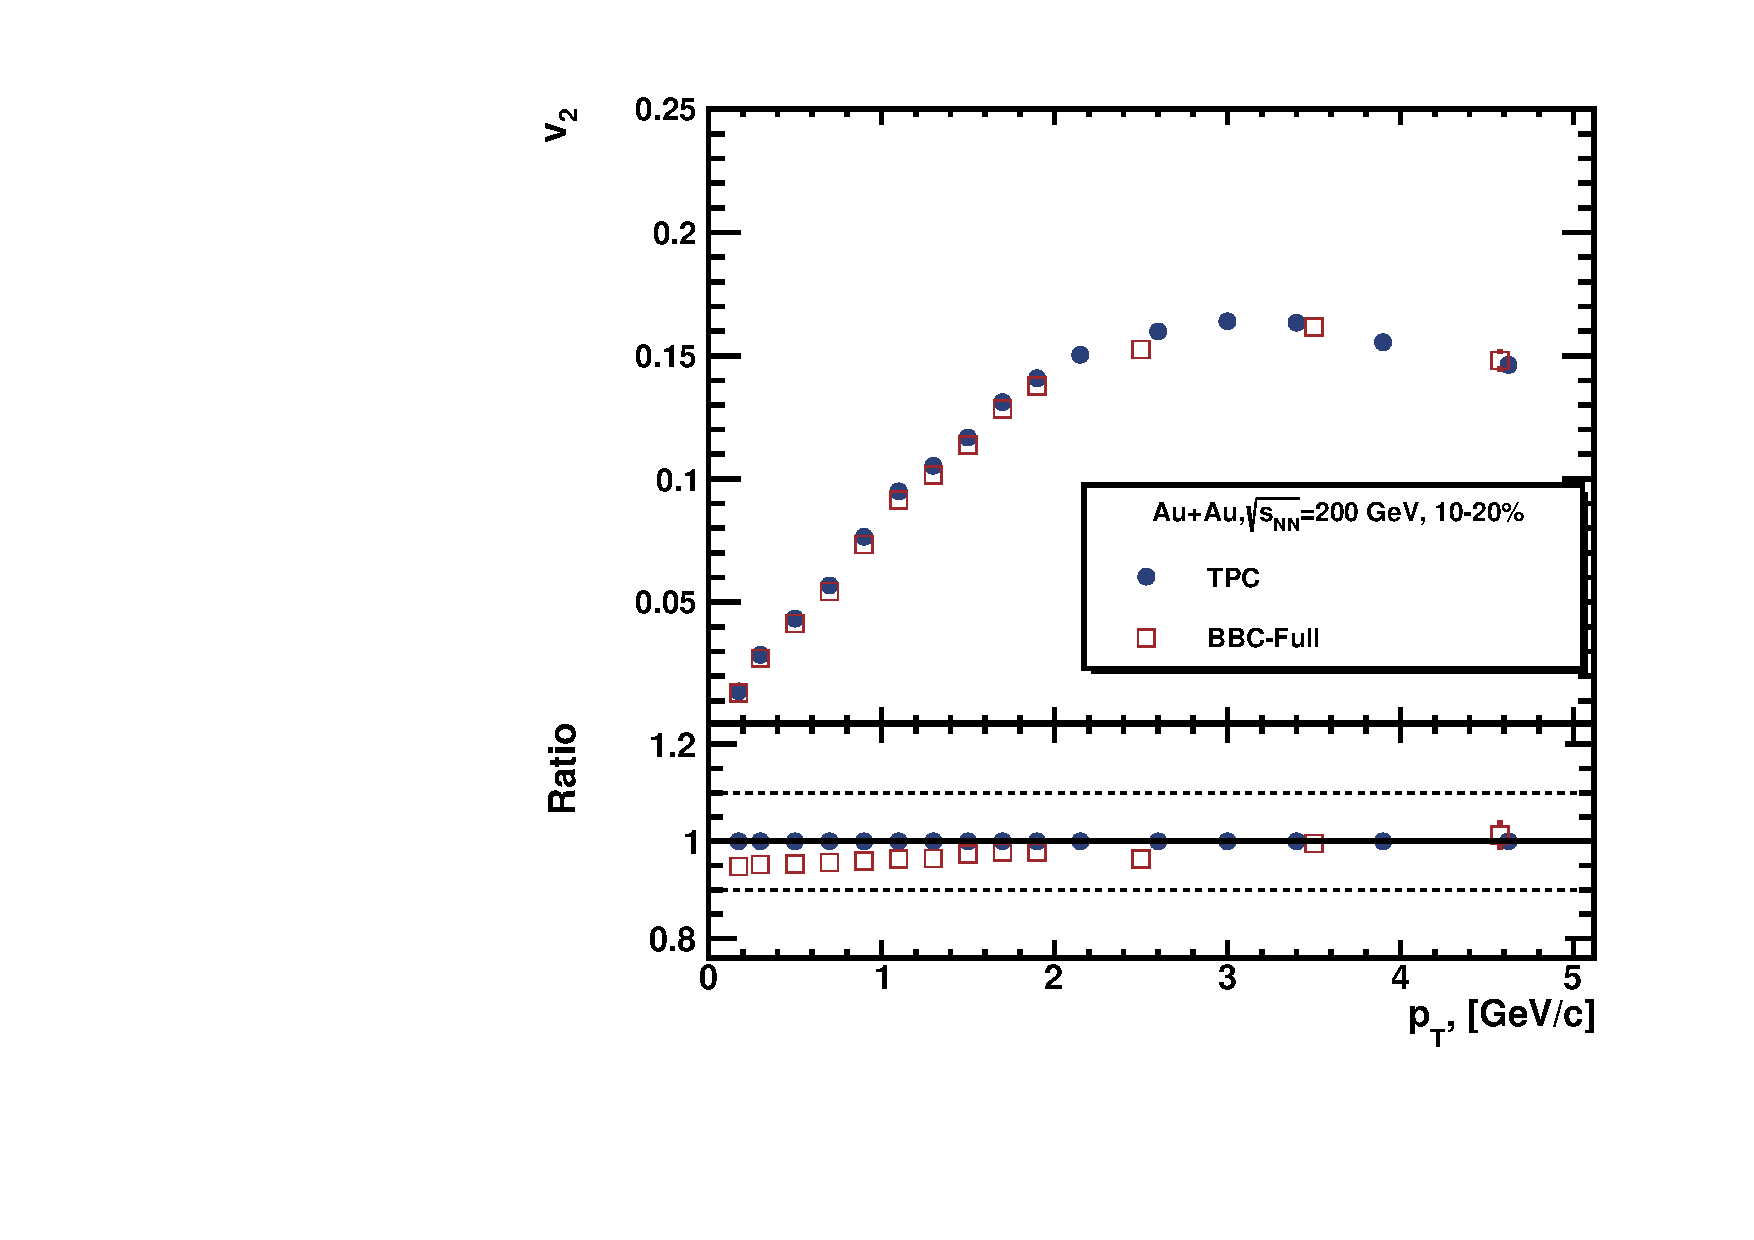
\includegraphics[width=1.\linewidth]{Figures/v2_CH_BBC_pt_cent2.pdf}
        %\caption{b}
    \end{subfigure}
    \\
    \begin{subfigure}{.49\textwidth}
        \centering
        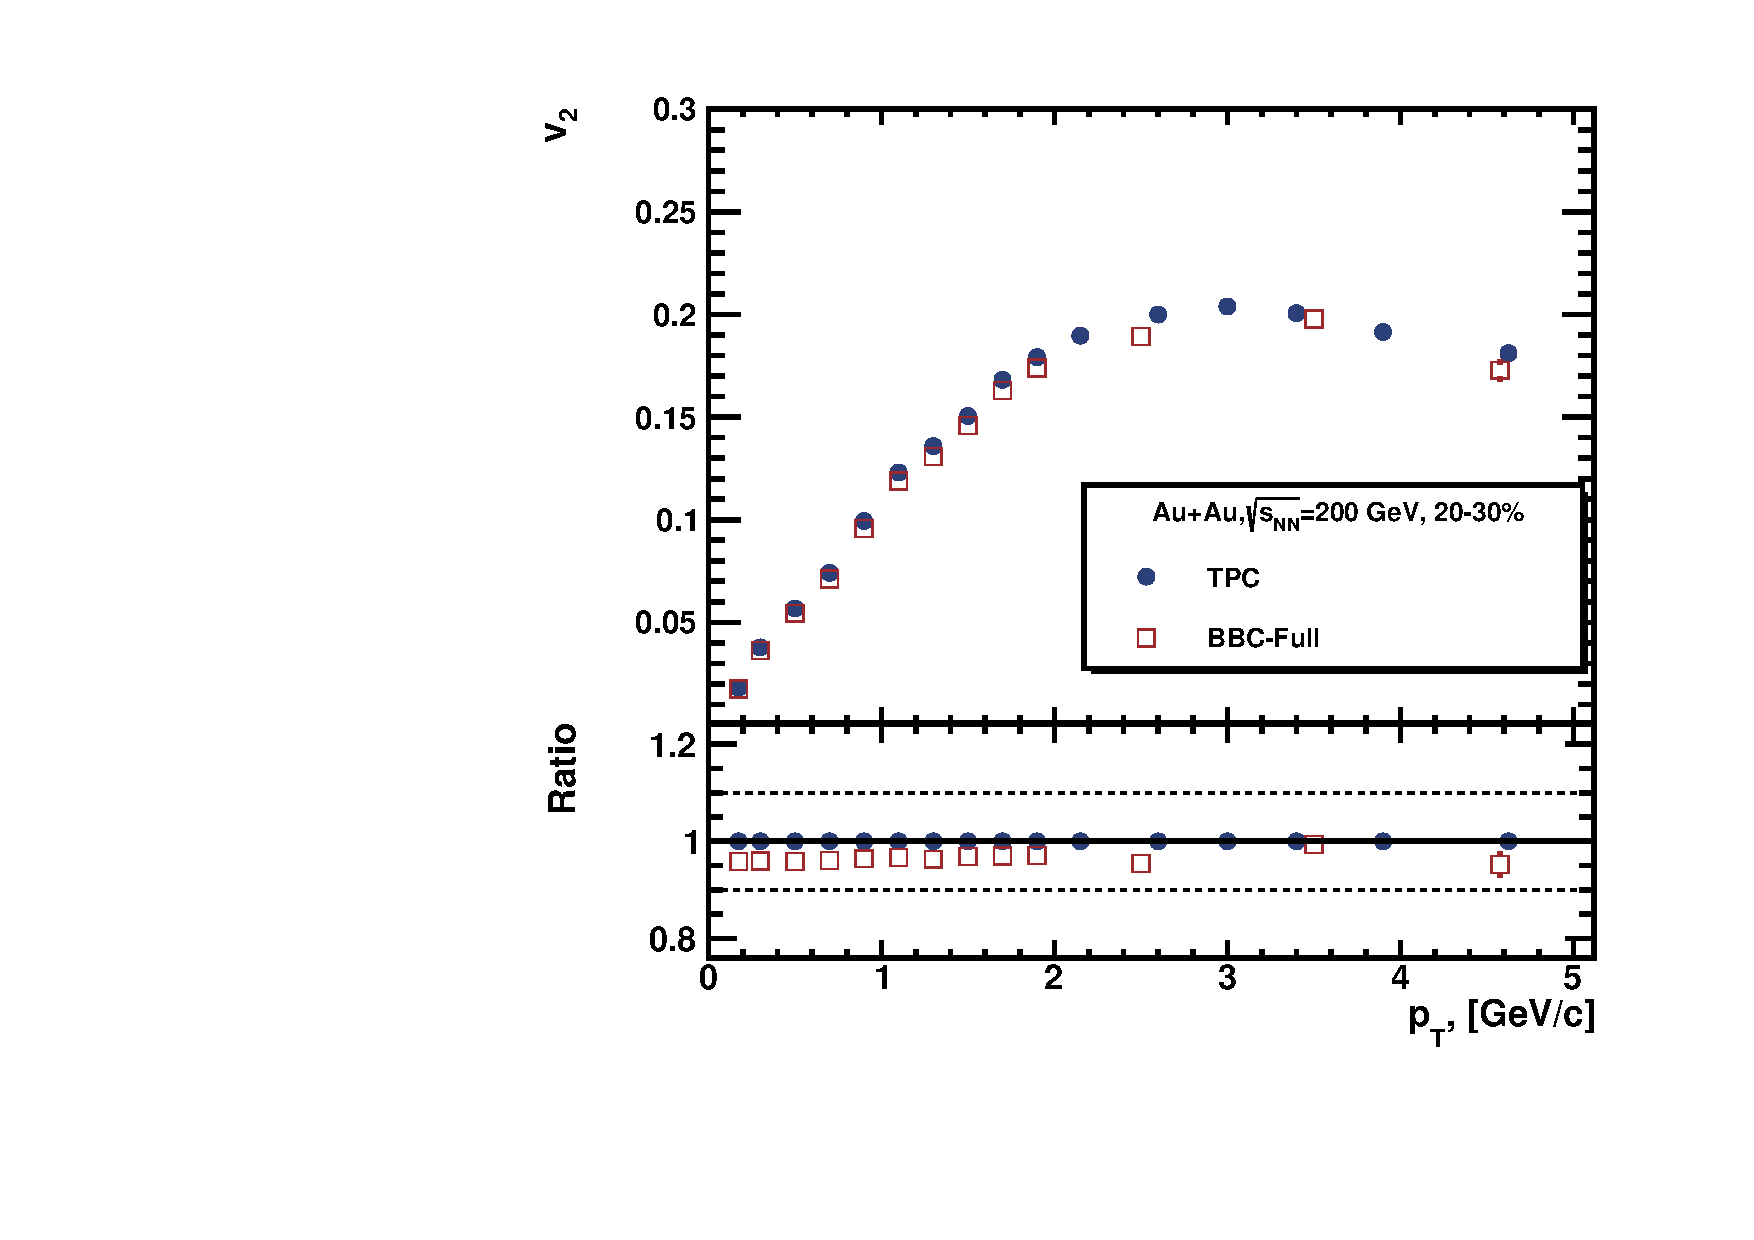
\includegraphics[width=1.\linewidth]{Figures/v2_CH_BBC_pt_cent3.pdf}
        %\caption{a}
    \end{subfigure}
    \begin{subfigure}{.49\textwidth}
        \centering
        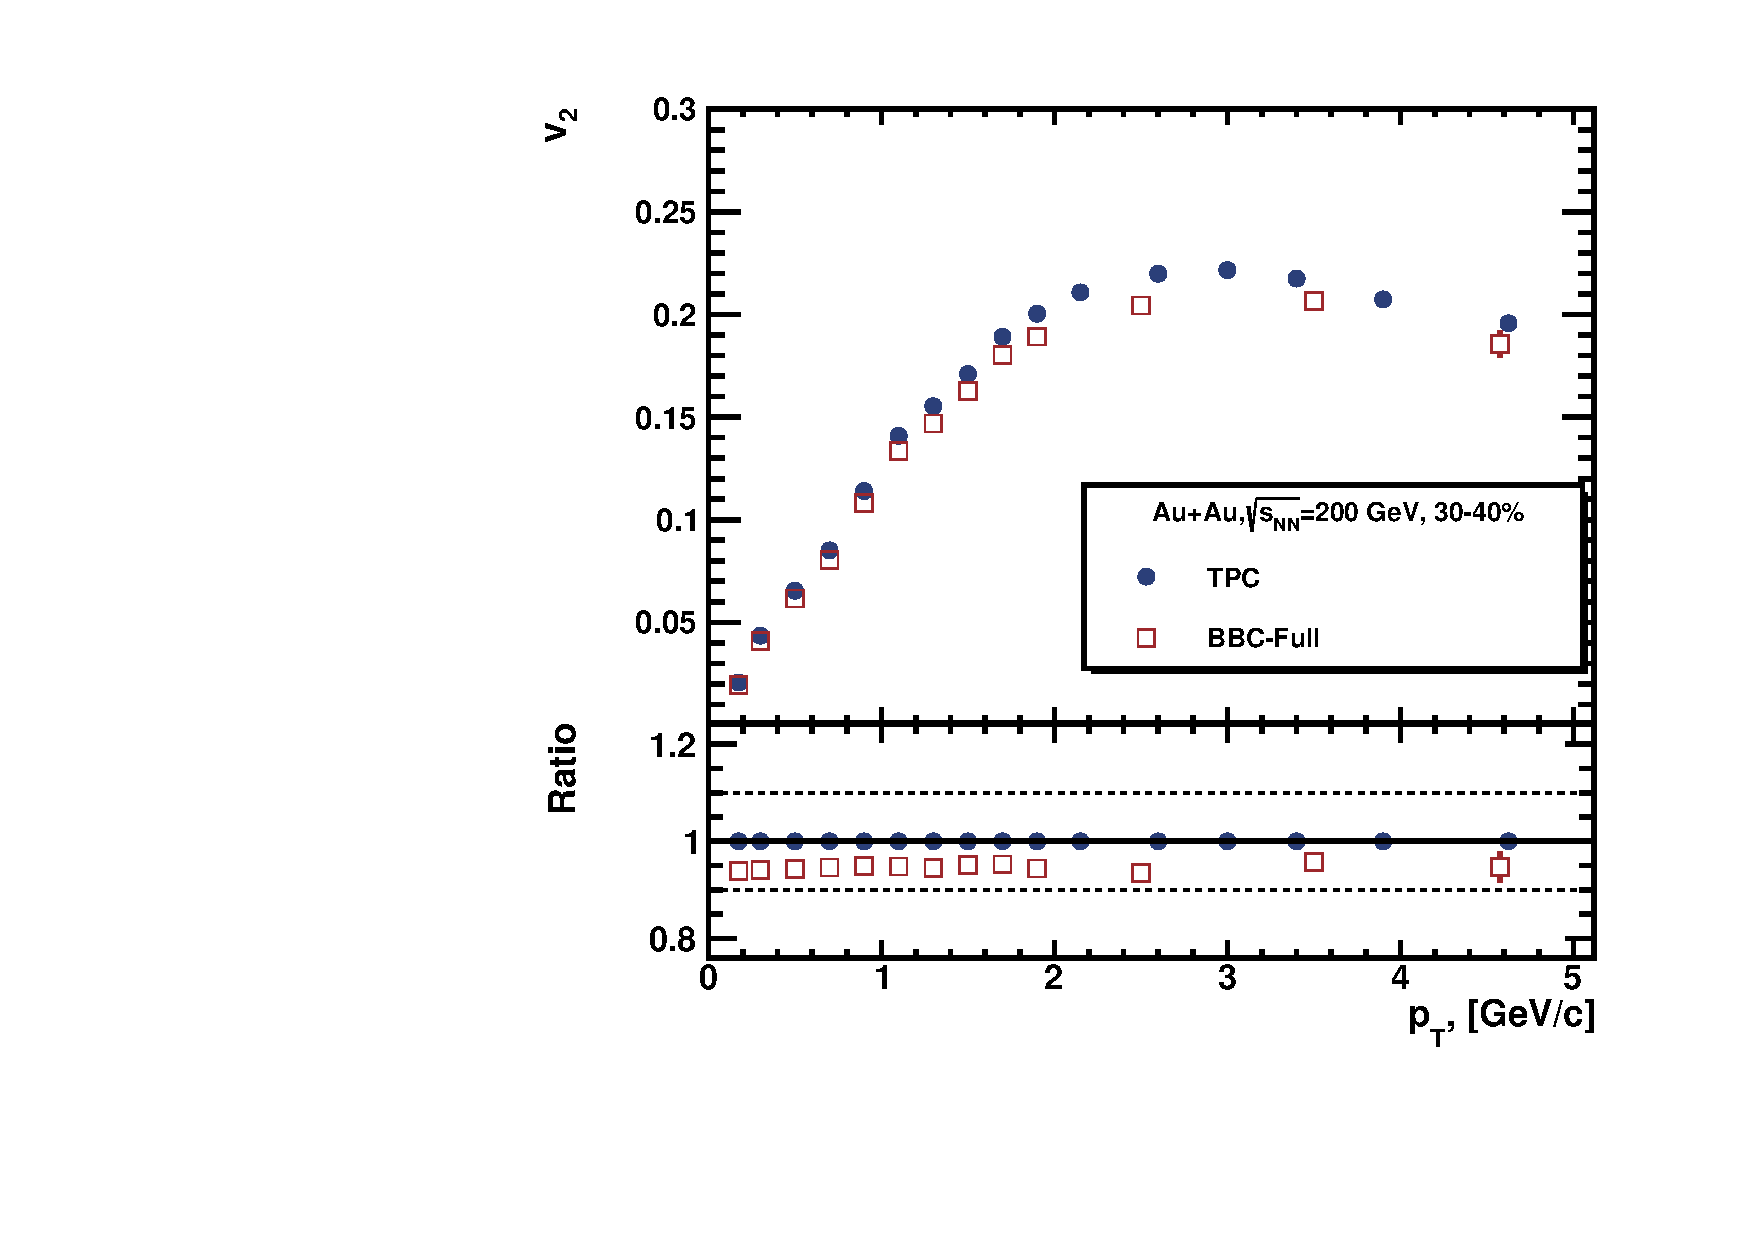
\includegraphics[width=1.\linewidth]{Figures/v2_CH_BBC_pt_cent4.pdf}
        %\caption{b}
    \end{subfigure}
    \label{fig:v2_BBC_CH}
    \caption{Charged hadron $v_2(p_T)$ for 5-10\% (upper left), 10-20\% (upper right), 20-30\% (bottom left) and 30-40 \% (bottom right) centrality classes in \AuAu\ collisions at \sNN\ = 200 GeV. Results gained with \BBC\ event-plane were compared with the \TPC\ event-plane ones.}
\end{figure}

\FloatBarrier
\subsubsection{3 sub-event method}

\begin{figure}[ht]
    \begin{subfigure}{.49\textwidth}
        \centering
        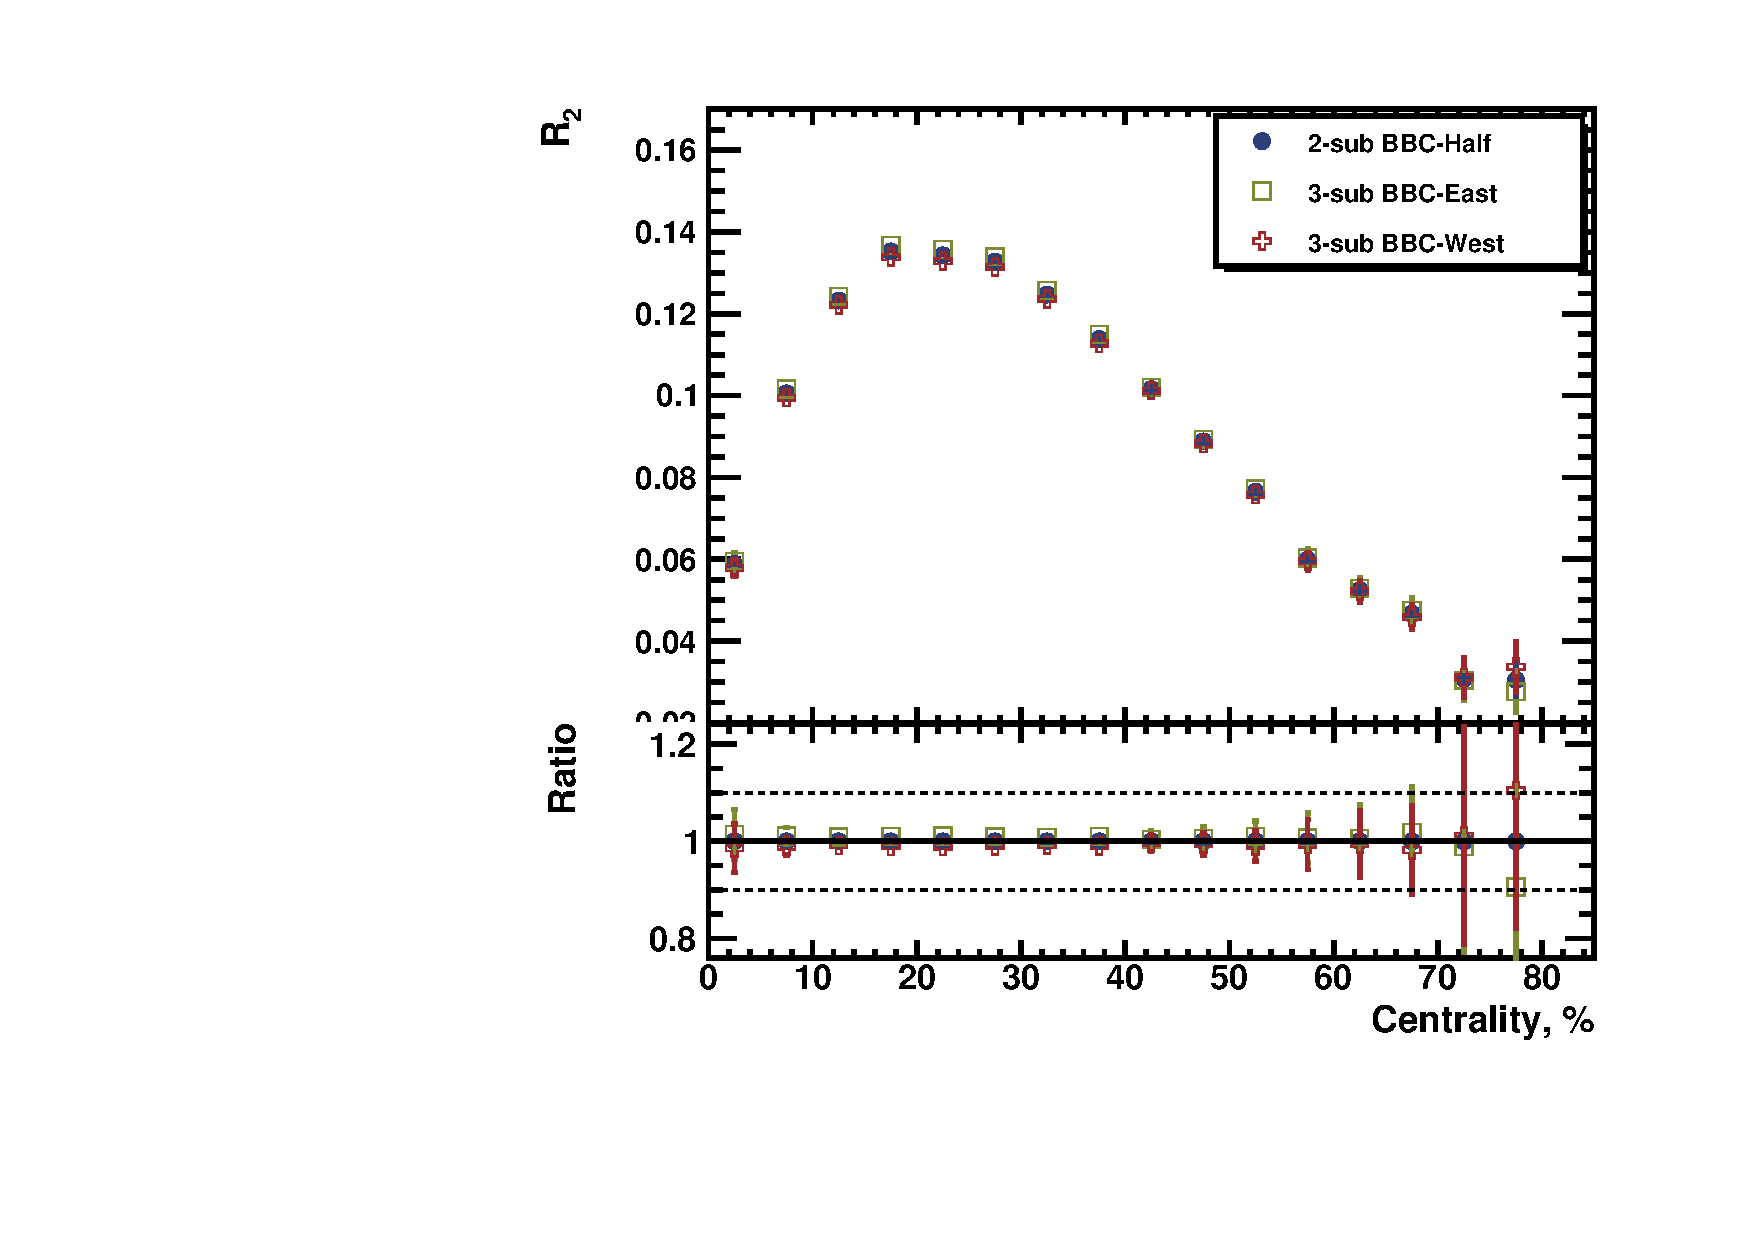
\includegraphics[width=1.\linewidth]{Figures/c_Res3sub2.pdf}
        %\caption{a}
    \end{subfigure}
    \begin{subfigure}{.49\textwidth}
        \centering
        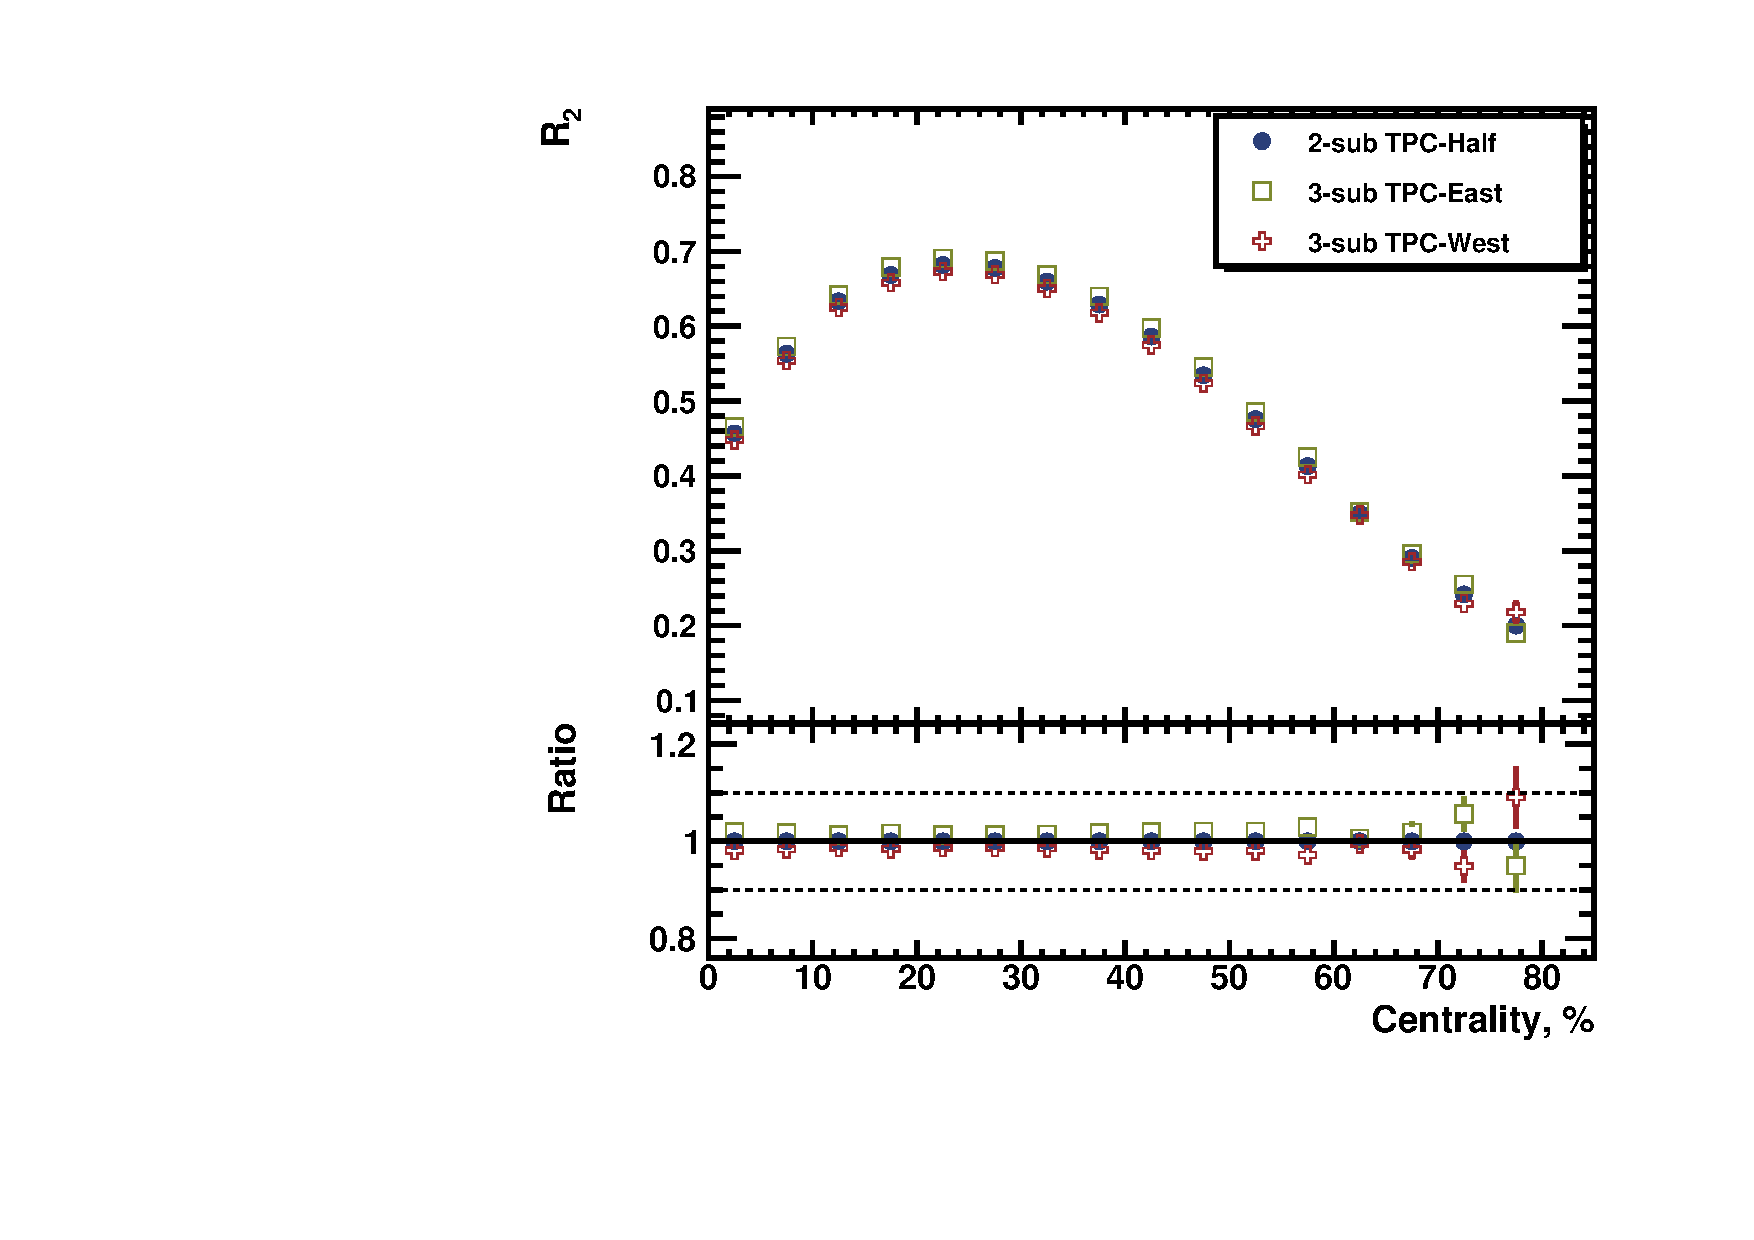
\includegraphics[width=1.\linewidth]{Figures/c_Res3sub3.pdf}
        %\caption{b}
    \end{subfigure}
    \label{fig:Res_3sub}
    \caption{The event-plane resolution correction factor calculated for \AuAu\ collisions at \sNN\ = 200 GeV using 3 and 2 sub-events as a function of centrality.}
\end{figure}